\documentclass{article}
\usepackage{graphicx}
\usepackage{subcaption}
\usepackage{wrapfig}

\begin{document}
%picture in the same file as Tex
\includegraphics{doraemon1.jpg}
%complete path of picture
\includegraphics{C:/Users/11510/Desktop/Start_LaTex/doraemon1.jpg} %It seems that the relative path does not work.
%
%reserved file for pictures
\graphicspath{{C:/Users/11510/Desktop/Start_LaTex/Reserved file for pictures}}
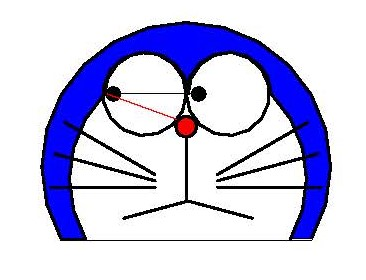
\includegraphics{doraemon2.jpg}

\includegraphics[scale=.3]{doraemon1.jpg}
\includegraphics[scale=.5]{doraemon1.jpg}
\includegraphics[scale=.7]{doraemon1.jpg}

\includegraphics[width=3cm]{doraemon1.jpg}
\includegraphics[width=.3\textwidth]{doraemon1.jpg}

\includegraphics[height=1cm]{doraemon1.jpg}
\includegraphics[height=.1\textheight]{doraemon1.jpg}

\includegraphics[scale=.3, angle=90]{doraemon1.jpg}%counterclockwise
\includegraphics[scale=.3, angle=-90]{doraemon1.jpg}%clockwise
\includegraphics[scale=.3, angle=90, origin=c]{doraemon1.jpg}%counterclockwise
\includegraphics[scale=.3, angle=-90, origin=c]{doraemon1.jpg}%clockwise

\fbox{\includegraphics{doraemon1.jpg}}
\setlength{\fboxsep}{.5cm}
\fbox{\includegraphics{doraemon1.jpg}}

This is a picture \includegraphics{doraemon1.jpg} inserted into the text.

This is a picture independent of the text.
\begin{figure}[htbp]
\centering
\includegraphics{doraemon1.jpg}
\caption{doraemon}
\end{figure}

\begin{figure}[htbp]
\centering
	\begin{subfigure}{.3\textwidth}%this argument of width is obligatory
	\centering
	\includegraphics[scale=.1]{doraemon1.jpg}
	\subcaption{doraemon(1)}
	\end{subfigure}
	%
	\begin{subfigure}{.3\textwidth}
	\centering
	\includegraphics[scale=.3]{doraemon1.jpg}
	\subcaption{doraemon(2)}
	\end{subfigure}
	%
	\begin{subfigure}{.3\textwidth}
	\centering
	\includegraphics[scale=.5]{doraemon1.jpg}
	\subcaption{doraemon(3)}
	\end{subfigure}	
\caption{subfigure}		
\end{figure}

\begin{wrapfigure}{l}{5cm}%Notice that this is the argument of width 
\centering
\includegraphics[scale=.3]{doraemon1.jpg}
\caption{picture inserted}
\end{wrapfigure}
Texte texte texte texte texte texte texte
texte texte texte texte texte texte texte
texte texte texte texte texte texte...
Texte texte texte texte texte texte texte
texte texte texte texte texte texte texte
texte texte texte texte texte texte...
Texte texte texte texte texte texte texte
texte texte texte texte texte texte texte
texte texte texte texte texte texte...


\clearpage
\listoffigures
\end{document}